% =====================================================================
% Versão em português — ICITS'27 / Springer LNNS.
% Classe: llncs. Revisão: DUPLO-CEGO (anônimo).
% Tradução da versão em inglês (paper.tex), norma culta.
% =====================================================================
\documentclass[runningheads]{llncs}

\usepackage[T1]{fontenc}
\usepackage[utf8]{inputenc}
\usepackage[brazilian]{babel}
\usepackage{graphicx}
\usepackage{booktabs}
\usepackage{amsmath}
\usepackage{algorithm}
\usepackage{algpseudocode}
\usepackage[hidelinks]{hyperref}
\usepackage{placeins} % \FloatBarrier: evita que figuras pendentes sejam
                       % empurradas para depois das Referências

\begin{document}

% --- DUPLO-CEGO: sem nomes/afiliações na submissão --------------------
\title{A Estrutura Dirigida Revela um Gargalo de Acesso que Escapa à
Análise Não Dirigida: um Estudo em Grafos de Três Bairros do Rio de
Janeiro}

\titlerunning{Estrutura Dirigida e Gargalos de Acesso em Redes Viárias}

\author{Autor(es) Anônimo(s)}
\authorrunning{Anônimo}
\institute{Afiliação omitida para revisão duplo-cega}

\maketitle

% =====================================================================
\begin{abstract}
Este estudo exploratório modela as redes viárias de três bairros do Rio
de Janeiro como grafos dirigidos e ponderados a partir do OpenStreetMap,
perguntando se a estrutura dirigida revela um gargalo de acesso que a
análise não dirigida deixa passar, e se isso reflete geografia, não
tamanho. A contagem de rotas resultante poderia ajudar um órgão de
mobilidade ou de defesa civil a sinalizar um bairro com apenas uma
saída. Usando algoritmos clássicos (conectividade, Dijkstra,
Bellman--Ford, centralidade de intermediação, fluxo máximo de
Edmonds--Karp), comparamos uma península compacta (Urca) com duas
grandes malhas abertas de orla (Copacabana e Botafogo). Os indicadores
estruturais separam as duas malhas da Urca mas, uma vez corrigido um
erro de recorte que atribuía parte de Botafogo à Copacabana, deixam de
se parecer entre si. O corte mínimo entre dois nós satura em um em toda
parte; um fluxo máximo de cada núcleo até suas portas de acesso
administrativas reais, por sua vez, ordena os casos: uma porta para a
Urca, dezoito para Copacabana, dezesseis para Botafogo. O gargalo é,
portanto, específico da geografia da península, não do seu tamanho, e
não se generaliza para bairros grandes. Todo o código e os dados são
abertos e reprodutíveis.

\keywords{Mobilidade urbana \and Grafos dirigidos \and Conectividade
forte \and Centralidade de intermediação \and Fluxo máximo \and Redes
viárias \and OpenStreetMap.}
\end{abstract}

% =====================================================================
\section{Introdução}
\label{sec:intro}

Redes viárias são naturalmente modeladas como grafos cujos vértices são
interseções e cujas arestas são trechos de rua. A direção do modelo
importa: a regulamentação de mão única pode deixar uma interseção
alcançável sem oferecer caminho de volta, distinção que um modelo não
dirigido é incapaz de expressar. Este artigo é um estudo exploratório
que caracteriza as redes viárias de três bairros do Rio de Janeiro e
testa uma única pergunta norteadora: a estrutura dirigida revela um
gargalo de acesso que a visão não dirigida deixa passar, e esse gargalo
é uma propriedade da \emph{geografia} do bairro, e não do seu
\emph{tamanho}?

Para separar geografia de tamanho, comparamos um bairro compacto e
geograficamente restrito, a Urca (uma península alcançada a partir do
restante da cidade por um único corredor), com duas grandes malhas
abertas de orla, Copacabana e Botafogo. As duas malhas grandes funcionam
como casos de comparação: se o padrão da Urca fosse apenas um artefato
de sua pequena escala, os indicadores acompanhariam o tamanho; se a
origem for geográfica, a Urca deve se destacar das duas malhas grandes.
Copacabana é de particular interesse porque seu acesso ao restante da
cidade é popularmente associado a um pequeno número de túneis, o que a
torna uma candidata plausível a um gargalo estrutural severo.

Além da questão algorítmica, o fluxo de acesso tem uma leitura prática
direta: o número de rotas independentes que um bairro perderia antes de
se tornar inalcançável por via terrestre, útil ao planejar diante de uma
enchente, um deslizamento ou a interdição de um túnel.

As contribuições deste trabalho são: (i) um \emph{pipeline} totalmente
reprodutível que constrói grafos viários dirigidos e ponderados a partir
do OpenStreetMap, confere sua extensão em relação a fronteiras
administrativas oficiais e analisa sua conectividade, centralidade e
fluxo; (ii) uma caracterização comparativa de três bairros reais,
mostrando que os indicadores estruturais tradicionais não os distinguem
ao longo de um eixo de gargalo; e (iii) um fluxo máximo do núcleo de cada
bairro até suas portas de acesso administrativas reais que os distingue,
diferente do corte mínimo entre dois nós. Mantemos deliberadamente a análise
restrita a $n=3$ casos contrastantes e interpretamos os resultados como
ilustrativos, não como uma afirmação estatisticamente generalizável.

% =====================================================================
\section{Trabalhos Relacionados}
\label{sec:related}

Extrair um grafo roteável a partir do OpenStreetMap e simplificar sua
topologia (contraindo os pontos de forma que são meras curvas de uma rua
em arestas únicas entre interseções verdadeiras) é prática consolidada,
popularizada por ferramentas como o OSMnx~\cite{boeing}; seguimos a
mesma construção e simplificação em um \emph{pipeline} compacto e
reprodutível, verificado em relação à biblioteca \texttt{networkx}.

A conectividade dispõe de um ferramental clássico para grafos não
dirigidos: pontes e pontos de articulação, calculados em tempo linear
pela busca em profundidade de Tarjan~\cite{tarjan1972depth}, identificam
as arestas e os vértices cuja remoção desconecta a rede. Essas primitivas
respondem se dois pontos permanecem mutuamente alcançáveis quando uma rua
é fechada, mas são cegas à direção. Italiano et
al.~\cite{italiano2012finding} as generalizaram para grafos dirigidos
como \emph{pontes fortes} e \emph{pontos de articulação fortes}, cuja
remoção aumenta o número de componentes fortemente conexas, e propuseram
algoritmos de tempo linear; as noções fortes captam se é possível ir e
voltar, não apenas alcançar.

Essa distinção não é apenas teórica para redes viárias, nas quais a
regulamentação de mão única é predominante (74--93\% dos trechos em
nossos casos). Ferramentas como o OSMnx~\cite{boeing} constroem grafos
viários dirigidos, mas estudos de conectividade e resiliência costumam
reduzi-los ao grafo não dirigido ou a resumos topológicos
agregados~\cite{corcoran2021persistent}, confundindo ``alcançável'' com
``alcançável e capaz de retornar'' e ocultando o efeito da direção.
Aplicamos as noções fortes a bairros reais, apresentamos lado a lado os
retratos fraco (não dirigido) e forte, e quantificamos o quanto o núcleo
fortemente conexo se reduz sob a direção --- uma lacuna que a análise não
dirigida não é capaz de enxergar. Privilegiamos a transparência em
detrimento da complexidade assintótica: em vez do algoritmo de tempo
linear de Italiano, recalculamos as componentes fortes após a remoção de
cada elemento candidato, restritas ao núcleo forte gigante, o que roda em
segundos nessa escala (dezenas a algumas centenas de interseções) -- uma
escolha de simplicidade, não uma alegação de escalabilidade.

Um amplo conjunto de trabalhos localiza pontos críticos em redes viárias
por meio de centralidade, sobretudo a de
intermediação~\cite{kirkley2018betweenness,halavachou2021uncovering}, e
por meio de modelos de gargalos
viários~\cite{stepanchuk2020modelling}. Uma tradição bem mais antiga, a
sintaxe espacial (\emph{space syntax}), lê a acessibilidade a partir de
medidas configuracionais como integração e escolha, calculadas sobre o
mapa axial ou de segmentos de um assentamento~\cite{hillier1984social}.
Ambas as tradições resumem uma rede a um único escore por vértice;
nenhuma delas responde diretamente quantas rotas \emph{independentes}
ligam duas regiões, a pergunta que importa antes de fechar uma rua. Nós,
em vez disso, lemos os
gargalos por meio de fluxo máximo / corte mínimo, que conta
explicitamente as rotas disjuntas por ruas e é comparável, em espírito, a
qualquer uma das abordagens agregadas, ainda que com granularidade mais
grosseira.

A resiliência de redes urbanas tem sido estudada como a degradação do
serviço sob falha. Ganin et al.~\cite{ganin2017resilience}, em quarenta
áreas urbanas dos Estados Unidos, constatam que eficiência e resiliência
variam de forma independente; nossa comparação não permite testar isso
diretamente, mas é compatível: a Urca não é ineficiente, mas é,
disparadamente, a mais frágil dos três casos. Avaliações baseadas em topologia simulam
falhas aleatórias e direcionadas para classificar elementos
críticos~\cite{rouhana2020,alatristasalas2019}; Ientile et
al.~\cite{ientile2022measuring} formalizam um índice de perda de
serviço; e uma abordagem topológica~\cite{corcoran2021persistent}
descreve a forma das redes viárias. Medimos a resiliência de modo
concreto, como o número de pares origem--destino que perdem toda a
conexão quando um único elemento forte é removido, e relacionamos o
custo de um desvio forçado à literatura sobre rotas
alternativas~\cite{silver2018tuned}. Diante desse panorama, a maioria
das análises trata a rede como não dirigida ou a resume por meio de um
escore agregado; poucas isolam o efeito da direção sobre a conectividade
de acesso e o contrastam entre bairros de geografia distinta, que é a
lacuna que este artigo explora.

% =====================================================================
\section{Metodologia}
\label{sec:method}

\subsection{Dados e Construção do Grafo}
\label{sec:data}

Para cada bairro, consultamos as vias trafegáveis (\texttt{highway} das
classes \emph{motorway} a \emph{residential}) dentro de um retângulo
delimitador (\emph{bounding box}) junto à API Overpass do OpenStreetMap,
e armazenamos em cache a resposta bruta para que a análise seja
reprodutível \emph{offline}. Cada trecho de rua torna-se um arco dirigido
que respeita sua \emph{tag} \texttt{oneway}: uma rua de mão dupla gera
dois arcos opostos; uma rua de mão única, um único arco. Pontos de forma
de grau dois são contraídos, de modo que os vértices sejam interseções
verdadeiras e as arestas sejam as ruas entre elas; sem essa etapa, cada
curva de uma rua se tornaria um falso ponto de articulação. As
coordenadas são projetadas em metros, e cada aresta é ponderada por seu
tempo de percurso, calculado a partir do comprimento e de uma velocidade
padrão por classe de via quando o OpenStreetMap não informa
\texttt{maxspeed}. A Figura~\ref{fig:construction} ilustra a conversão
do mapa para o grafo dirigido.

\begin{figure}[t]
\centering
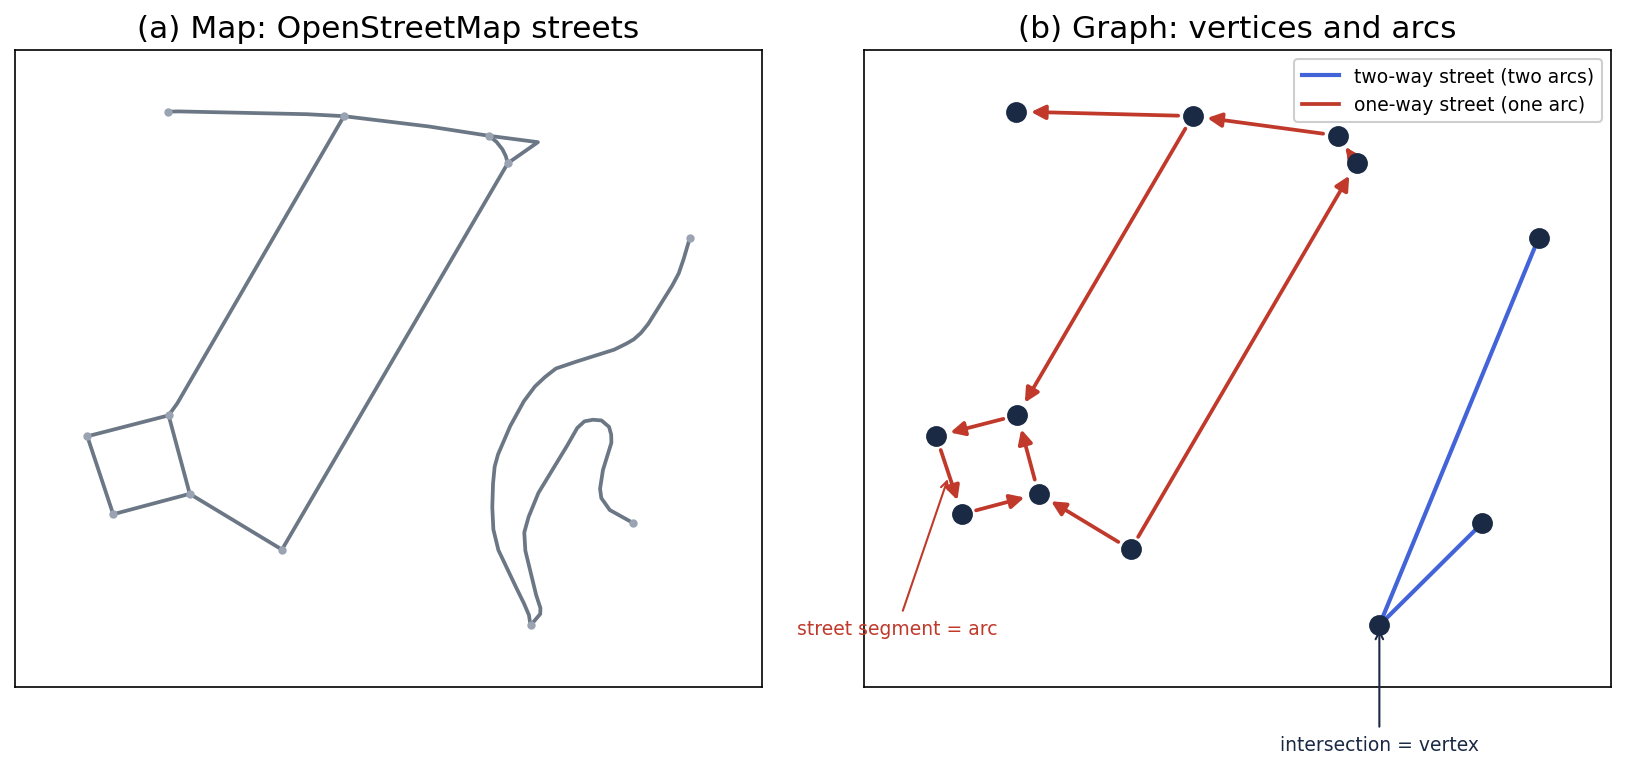
\includegraphics[width=\textwidth]{Figures/fig_construction.png}
\caption{Do mapa ao grafo dirigido: interseções tornam-se vértices e
trechos de rua tornam-se arcos; uma rua de mão única gera um único arco
(seta), uma rua de mão dupla gera dois arcos opostos.}
\label{fig:construction}
\end{figure}

Um retângulo delimitador traçado manualmente é uma escolha de modelagem,
e constatamos que essa escolha tem consequências. O retângulo de
Copacabana foi originalmente traçado para manter seus dois túneis
rodoviários como arestas internas, estendendo-se para o norte, além da
fronteira administrativa com Botafogo. A conferência de cada interseção
em relação ao polígono oficial do bairro (Instituto Pereira Passos /
Data.Rio, camada \emph{Limite de Bairros}~\cite{ipp_bairros}) mostrou
que 158 de suas 496 interseções, e 155 de seus trechos de rua,
situavam-se, na verdade, dentro do território de Botafogo: as duas
redes publicadas compartilhavam 143 interseções idênticas do
OpenStreetMap. Por isso, passamos a usar o retângulo manual apenas como
envelope de busca, unido ao retângulo delimitador do próprio polígono
oficial para garantir cobertura total, e recortamos o grafo resultante
pelo polígono oficial antes de qualquer análise. Urca e Botafogo não
precisaram dessa correção: no máximo quatro de suas interseções ficam
fora do próprio polígono, e nenhum de seus números publicados se altera.
Toda figura e tabela referentes a Copacabana neste artigo refletem a
rede corrigida e recortada pelo polígono, com 345 interseções
(Tabela~\ref{tab:redes}), e não as 496 originais.

\begin{table}[t]
\centering
\caption{Redes após a simplificação topológica (OpenStreetMap);
Copacabana está recortada pelo seu polígono administrativo oficial.}
\label{tab:redes}
\begin{tabular}{lrrr}
\toprule
 & Urca & Copacabana & Botafogo \\
\midrule
Interseções ($V$)                     & 60   & 345  & 398 \\
Trechos de rua                        & 89   & 494  & 500 \\
Trechos de mão única (\%)             & 93,3 & 74,9 & 76,4 \\
Núcleo fortemente conexo ($V$)        & 37   & 331  & 341 \\
Fora do núcleo gigante (\% de $V$)    & 38,3 & 4,1  & 14,3 \\
\bottomrule
\end{tabular}
\end{table}

A Figura~\ref{fig:networks} mostra as três redes após a simplificação,
distinguindo trechos de mão única e de mão dupla. As duas malhas
residenciais da Urca, unidas por um único corredor de mão dupla, ficam
visíveis em contraste com as grandes malhas abertas de Copacabana e
Botafogo; esse corredor é a constrição de acesso analisada na
Seção~\ref{sec:results}.

\begin{figure}[t]
\centering
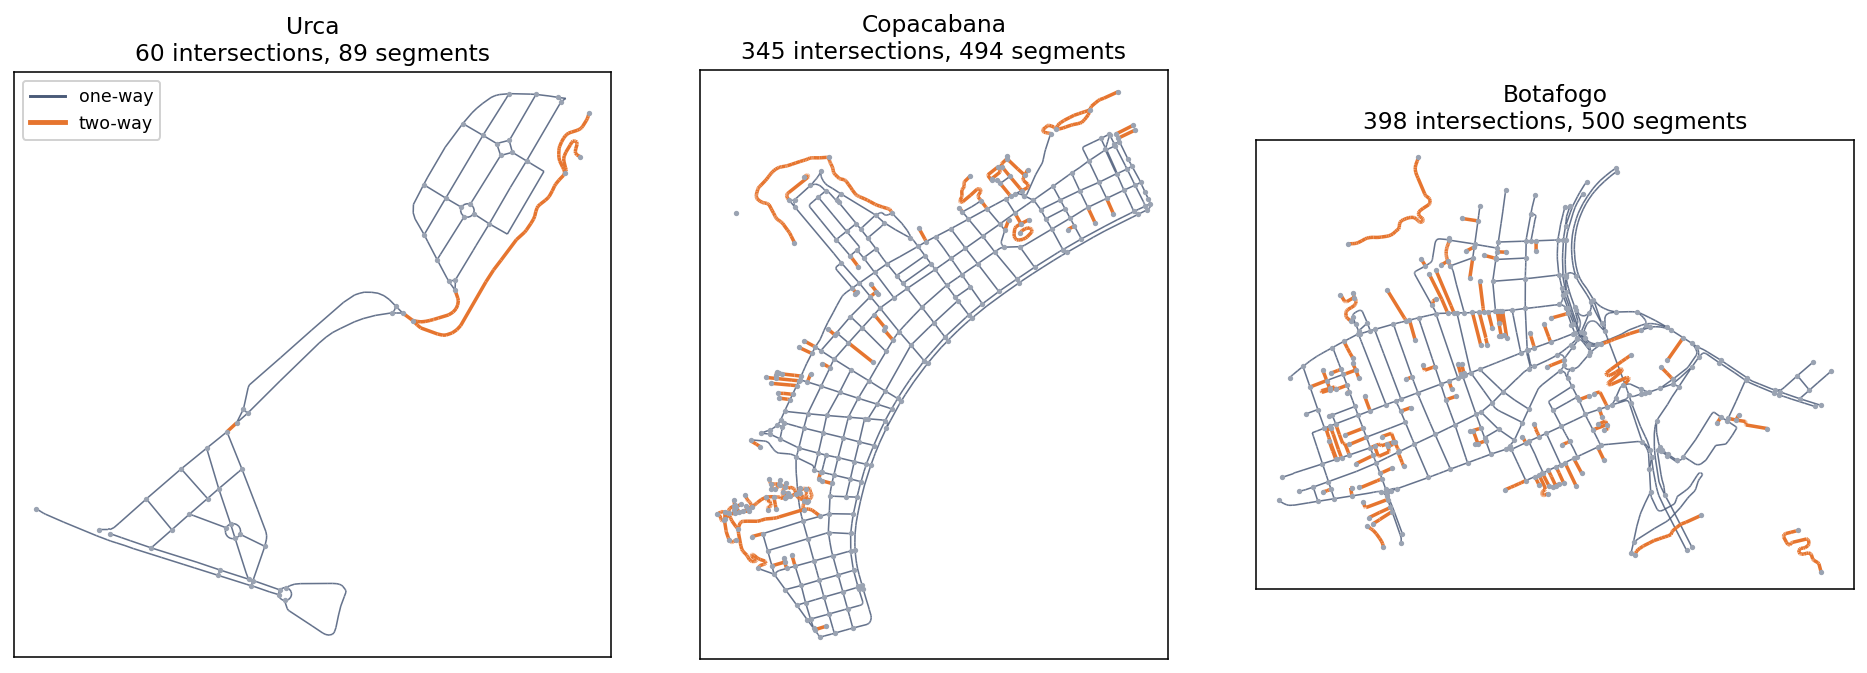
\includegraphics[width=\textwidth]{Figures/fig_networks.png}
\caption{As três redes dos bairros após a simplificação topológica (mão
única em escuro, mão dupla em laranja). A Urca é uma península compacta
cujas duas malhas se encontram em um único corredor de mão dupla;
Copacabana e Botafogo são grandes malhas abertas. O painel de Copacabana
reflete a rede corrigida e recortada pelo polígono.}
\label{fig:networks}
\end{figure}

\subsection{Conectividade, Caminhos Mínimos e Fluxo}
\label{sec:algos}

Todas as análises são executadas sobre um grafo dirigido e ponderado,
representado por lista de adjacência, e nossas implementações foram
verificadas em relação à biblioteca \texttt{networkx}. Componentes
conexas não dirigidas e componentes fortemente conexas dirigidas (CFC)
são encontradas por busca em largura, esta última pela interseção do
conjunto alcançável no grafo com o conjunto alcançável em seu reverso.
Pontes e pontos de articulação \emph{fracos} são calculados diretamente
a partir de sua definição, removendo o elemento e recontando as
componentes não dirigidas. Pontes e pontos de articulação \emph{fortes}
são obtidos de modo análogo no cenário dirigido: um elemento é forte
quando sua remoção divide o núcleo fortemente conexo gigante em mais de
uma CFC, seguindo as definições de Italiano et
al.~\cite{italiano2012finding}. Os caminhos mínimos usam
Dijkstra~\cite{dijkstra1959note} com \emph{heap} binário, verificado de
forma independente por Bellman--Ford~\cite{bellman1958routing}; uma rota
alternativa é o caminho mínimo recalculado após o bloqueio de um trecho
(Seção~\ref{sec:res-resil}). O fluxo máximo e o corte mínimo usam
Edmonds--Karp~\cite{edmonds1972theoretical} com capacidade unitária por
rua, de modo que o fluxo máximo entre dois pontos seja igual ao número
de rotas disjuntas por ruas entre eles, e o corte mínimo seja o menor
conjunto de ruas cujo fechamento os separa. A centralidade de
intermediação é calculada com o algoritmo de
Brandes~\cite{brandes2001faster} sobre o grafo dirigido, ponderando os
caminhos mínimos pelo tempo de percurso, de modo que o escore de um
vértice seja a fração dos pares origem--destino de tempo mínimo que
passam por ele.

\subsection{Fluxo de Acesso por Portas}
\label{sec:access-flow}

O corte mínimo entre duas interseções isoladas satura em um nas três
redes (Seção~\ref{sec:results}): como as malhas de mão única densa
contêm pontes não dirigidas por quase toda parte, quase todo par
origem--destino é separado por uma única aresta próxima a uma das
extremidades, bem antes de qualquer constrição geográfica.

Para medir o acesso ao restante da cidade, em vez de uma travessia
interna arbitrária, distinguimos o \emph{interior} de um bairro de suas
\emph{portas de acesso} (\emph{gateways}). Cada rede viária é extraída
com uma pequena margem além da própria fronteira do bairro (seu polígono
oficial, no caso de Copacabana; seu retângulo delimitador de busca, no
caso de Urca e Botafogo), suficiente para incluir a primeira interseção
além da fronteira em toda rua que a cruze. Um vértice é uma porta de
acesso se pelo menos uma de suas arestas incidentes cruza essa
fronteira; todo outro vértice é interior. O conjunto de portas de acesso
é, portanto, o conjunto de pontos pelos quais é fisicamente possível
deixar o bairro, e não um marco interno escolhido por uma heurística de
distância. Como uma porta de acesso pode admitir tráfego em apenas um
sentido, restringimos o interior e o conjunto de portas de acesso ao
maior componente \emph{não dirigido} do bairro, e não ao seu núcleo
fortemente conexo: uma saída de mão única ainda é uma saída real.

A região de origem é a fração $f$ ($f=0{,}2$) das interseções interiores
mais distantes, em número de arestas, da porta de acesso mais próxima,
ou seja, o núcleo do bairro. Uma superfonte alimenta a região de origem,
e o conjunto completo de portas de acesso alimenta um superssumidouro,
ambos com capacidade infinita, e o algoritmo de Edmonds--Karp é
executado entre eles sobre a rede de capacidade unitária. O valor
resultante, que chamamos de \emph{fluxo de acesso}, é o número de rotas
disjuntas por ruas entre o núcleo do bairro e suas saídas reais para o
restante da cidade (Seção~\ref{sec:res-access}); esse valor é estável
para $f \in [0{,}15, 0{,}25]$ nos três bairros e, no caso da Urca, para
uma margem de busca de fronteira entre 200 e 800\,m.

Isso substitui uma definição anterior, construída a partir de dois polos
internos encontrados por uma varredura dupla do grafo, que media a
travessia mais estreita ao longo do eixo mais alongado do bairro mas
nunca fazia referência à sua fronteira real; mantemos essa construção
apenas como verificação interna de que a região de origem e o conjunto
de portas de acesso nunca se sobrepõem.

% =====================================================================
\section{Resultados}
\label{sec:results}

\subsection{Os Indicadores Estruturais Não Separam os Casos}
\label{sec:res-struct}

A Tabela~\ref{tab:estrutural} apresenta os indicadores estruturais
dirigidos como proporções, já que as contagens brutas não são
comparáveis entre redes de tamanhos tão diferentes. As duas malhas
grandes permanecem distantes do regime da Urca, mas deixam de se
acompanhar de perto uma vez que Copacabana é corrigida para sua
fronteira oficial (Seção~\ref{sec:data}): Botafogo tem consideravelmente
mais pontes fortes (70,4\% de suas ruas do núcleo) e articulações fortes
(63,9\%) do que Copacabana (45,3\% e 54,1\%). A Urca também não se
destaca de forma decisiva nessas proporções (67,3\% de pontes fortes,
75,7\% de articulações fortes). A Figura~\ref{fig:urca-strong} mostra,
para a Urca, que os elementos fortes se concentram dentro da malha
residencial, e não em um único ponto de acesso. As proporções, portanto,
separam a Urca das duas malhas abertas, mas não separam as duas malhas
abertas entre si, um contraste desenvolvido na
Seção~\ref{sec:discussion}.

\begin{table}[t]
\centering
\caption{Indicadores estruturais dirigidos (normalizados); os valores de
Copacabana referem-se à rede corrigida e recortada pelo polígono.}
\label{tab:estrutural}
\begin{tabular}{lrrr}
\toprule
 & Urca & Copacabana & Botafogo \\
\midrule
Pontes fracas (\% dos trechos)          & 10,1 & 15,8 & 25,2 \\
Pontes fortes (\% das ruas do núcleo)   & 67,3 & 45,3 & 70,4 \\
Articulações fortes (\% do núcleo)      & 75,7 & 54,1 & 63,9 \\
\bottomrule
\end{tabular}
\end{table}

\begin{figure}[t]
\centering
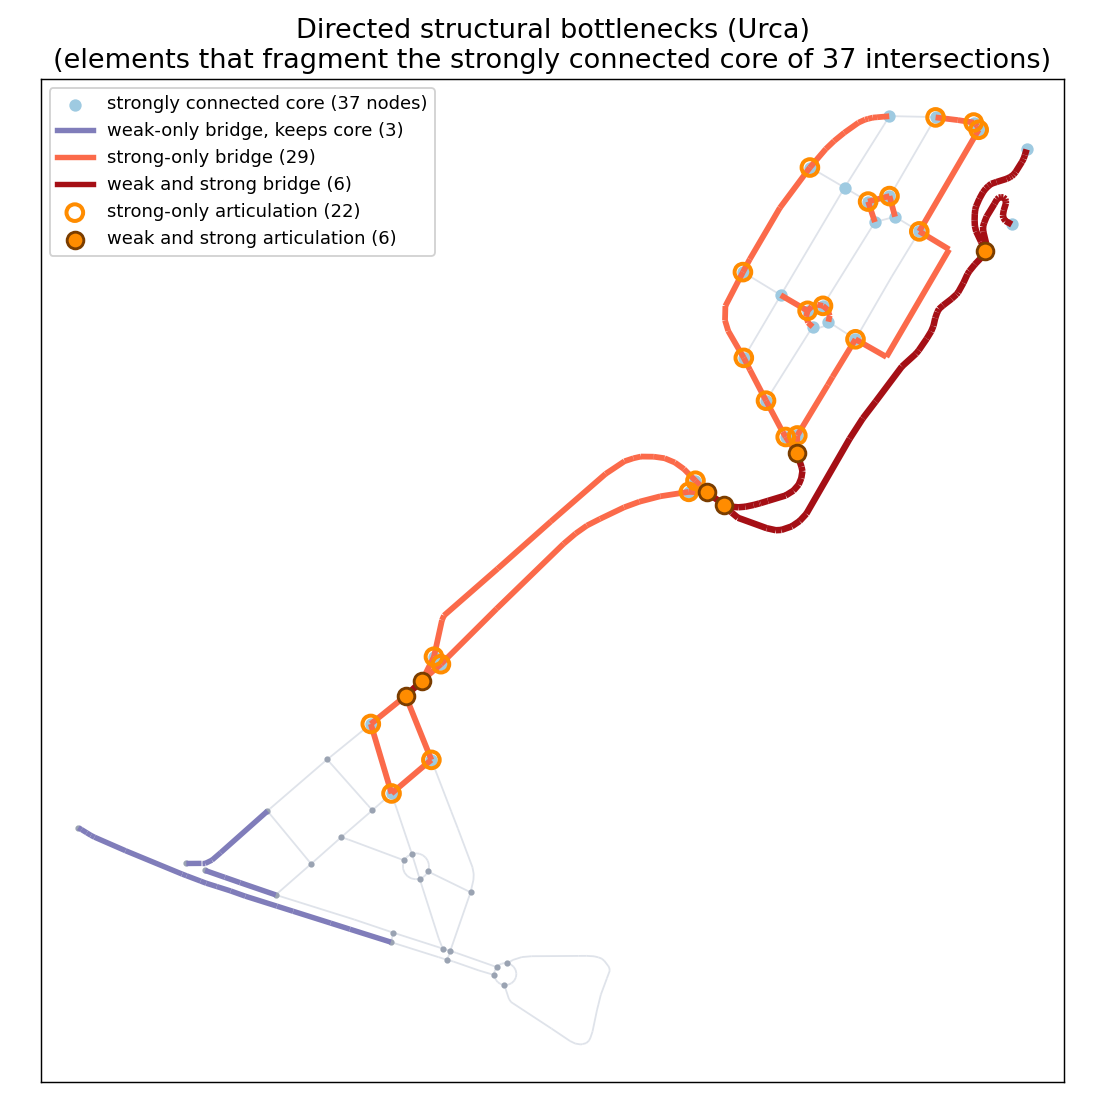
\includegraphics[width=0.72\textwidth]{Figures/fig_urca_strong.png}
\caption{Gargalos estruturais dirigidos na Urca: ruas cuja remoção
fragmenta o núcleo fortemente conexo (pontes fortes) e interseções com a
mesma propriedade (pontos de articulação fortes). Eles se situam
majoritariamente dentro da malha residencial, e não em um único ponto de
acesso.}
\label{fig:urca-strong}
\end{figure}

\subsection{O Corte Mínimo Entre Dois Nós Satura}
\label{sec:res-mincut}

Para uma origem e um destino bem conectados dentro do núcleo forte, o
corte mínimo de Edmonds--Karp é igual a um nos três bairros. A única
aresta de corte situa-se perto de uma das extremidades, e não em algum
estrangulamento geográfico: como a rede não dirigida tem pontes por toda
parte, um par origem--destino quase sempre tem uma única rua separadora
próxima a ele. O corte mínimo entre dois nós é, portanto, pouco
informativo sobre acesso; ele mede uma ponte local, não a conexão do
bairro com o restante da cidade.

\subsection{O Fluxo de Acesso por Portas Separa os Casos}
\label{sec:res-access}

O fluxo de acesso por portas da Seção~\ref{sec:access-flow} ordena os
casos (Tabela~\ref{tab:acesso}). A Urca tem uma única rota disjunta por
ruas entre seu núcleo e suas quatro portas de acesso reais ao restante
da cidade, valor estável para $f \in [0{,}15, 0{,}25]$ e para uma margem
de busca de fronteira entre 200 e 800\,m. Copacabana oferece dezoito
dessas rotas por meio de vinte e uma portas de acesso, estável na mesma
faixa de $f$; Botafogo oferece de quinze a dezesseis por meio de vinte e
oito, o único dos três valores com alguma sensibilidade a $f$, e ainda
assim uma ordem de grandeza acima da Urca em toda a faixa. Esse é o único
indicador que isola um gargalo de acesso, e ele não acompanha o tamanho:
Botafogo (seis a oito vezes maior que a Urca) e a Copacabana, agora bem
menor após a correção, oferecem ambos uma ordem de grandeza a mais de
rotas do que a Urca. O acesso de Copacabana não se reduz a seus dois
túneis: eles são apenas duas de suas vinte e uma portas de acesso, de
modo que ruas de superfície sustentam a maior parte de suas dezoito
rotas disjuntas.

\begin{table}[t]
\centering
\caption{Fluxo de acesso por portas: rotas disjuntas por ruas do núcleo
de cada bairro até suas portas de acesso administrativas reais
($f=0{,}2$; ver Seção~\ref{sec:access-flow} quanto à faixa de $f$ e,
para a Urca, à margem de busca de fronteira).}
\label{tab:acesso}
\begin{tabular}{lrrr}
\toprule
 & Urca & Copacabana & Botafogo \\
\midrule
Portas de acesso identificadas         & 4    & 21             & 28 \\
Fluxo de acesso (rotas)                & 1    & 18             & 16 \\
Intermediação máxima (\% dos pares)    & 52,2 & 27,8 & 22,5 \\
Interpretação                          & corredor único & malha aberta & malha aberta \\
\bottomrule
\end{tabular}
\end{table}

\subsection{A Intermediação Se Concentra em Uma Interseção na Urca}
\label{sec:res-betweenness}

A centralidade de intermediação dirigida, ponderada pelo tempo de
percurso, é compatível com a leitura do fluxo de acesso nos três bairros
(Figura~\ref{fig:betweenness}). Na Urca, uma única interseção está
presente em 52\% de todos os pares origem--destino de tempo mínimo,
exatamente a que fica no gargalo do corredor de acesso. Copacabana e
Botafogo não têm um vértice tão dominante: suas interseções mais
centrais alcançam 27,8\% e 22,5\%, respectivamente, com a carga
distribuída ao longo de um eixo arterial em forma de Y em Copacabana e
ao longo de eixos paralelos em Botafogo. O valor de Copacabana fica um
pouco acima do de Botafogo, mais um indicador em que as duas malhas
abertas deixam de se acompanhar exatamente depois da correção de
Copacabana (Seção~\ref{sec:discussion}). Reportamos o máximo, e não um
índice de concentração, porque este último é confundido pelo tamanho do
núcleo (um núcleo pequeno eleva a mediana e reduz a desigualdade
independentemente da geografia); o máximo, já normalizado pelo número de
pares, é comparável entre tamanhos distintos e volta a isolar a Urca.

\begin{figure}[t]
\centering
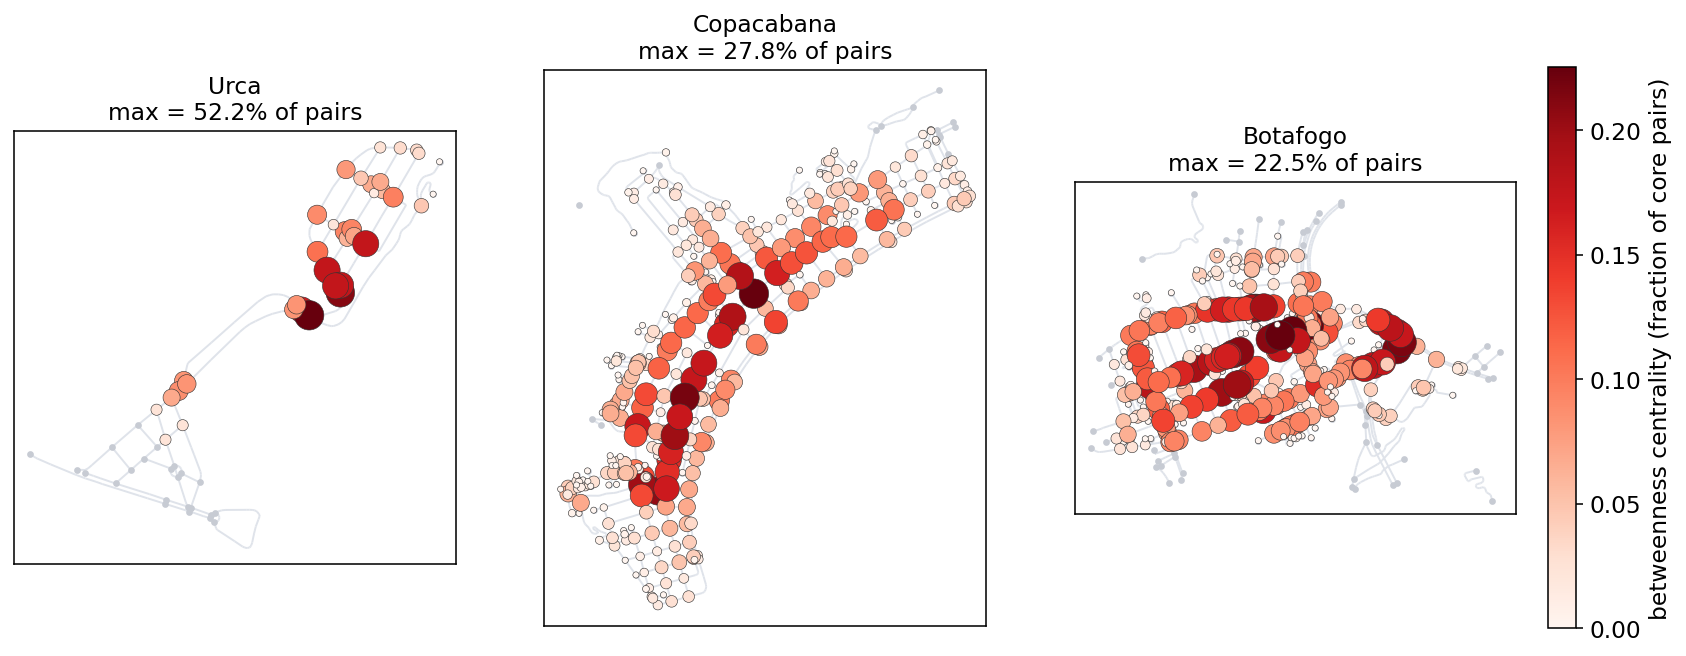
\includegraphics[width=\textwidth]{Figures/fig_betweenness.png}
\caption{Centralidade de intermediação dirigida (caminhos de tempo
mínimo, núcleo forte). O corredor de acesso da Urca é um único ponto
crítico; a carga de Copacabana se concentra ao longo de um eixo arterial
em forma de Y, e a de Botafogo ao longo de eixos paralelos, ambos com um
máximo bem mais baixo do que o da Urca.}
\label{fig:betweenness}
\end{figure}

\subsection{Resiliência do Núcleo Forte}
\label{sec:res-resil}

Medimos a resiliência de modo exaustivo, fechando cada ponte forte ou
articulação forte por vez e contando, sobre todos os pares ordenados do
núcleo, quantos perdem toda a conexão. Na Urca (1.332 pares do núcleo),
a ponte forte mediana desconecta 138 pares, e a pior, 644; a articulação
forte mediana desconecta 219, e a pior, 694. Em Copacabana (109.230
pares, na rede corrigida), a ponte forte mediana desconecta 660 pares, e
a pior, 14.280; em Botafogo (115.940 pares), 1.016 e 18.122,
respectivamente. A \emph{fração} do núcleo isolada é muito maior na Urca
(mediana de 10,4\% para pontes fortes, contra 0,6\% e 0,9\% nas malhas
grandes), mas isso é, em parte, um efeito de escala: um único elemento
removido corta uma fatia maior de um núcleo pequeno, de modo que as
contagens absolutas e o tamanho do núcleo na Tabela~\ref{tab:redes}
devem ser lidos em conjunto. O ponto qualitativo é robusto: em todos os
bairros, nenhuma ponte forte é inofensiva, a menos danosa ainda isola um
número não trivial de pares, e o impacto de um elemento não é uma
propriedade fixa, mas depende de qual par é considerado.

Além da conectividade binária, um desvio forçado tem um custo
mensurável. Recalcular a rota mais curta após bloquear, ao longo dela,
um trecho que não seja ponte aumenta o tempo de percurso em 13,6\% na
Urca, 5,1\% em Copacabana e 6,0\% em Botafogo. Essas mesmas rotas também
atravessam trechos que são, eles próprios, pontes fortes (3, 4 e 1,
respectivamente): fechar qualquer um deles não admite desvio algum,
apenas a desconexão já quantificada acima.

% =====================================================================
\section{Discussão}
\label{sec:discussion}

Lidos em conjunto, os indicadores continuam separando a Urca das duas
malhas abertas, mas deixam de agrupar Copacabana e Botafogo tão de perto
quanto sugeriria uma leitura não corrigida. A Urca é o caso restrito:
93,3\% de seus trechos são de mão única, essa direcionalidade remove
38,3\% de suas interseções do núcleo forte, e uma única rota disjunta
por porta de acesso liga seu núcleo ao restante da cidade, com uma
interseção presente em 52\% de suas rotas de tempo mínimo. Copacabana e
Botafogo são, ambos, casos abertos no sentido que importa para o acesso:
nenhum deles se assemelha ao padrão de porta única da Urca, oferecendo
dezoito e dezesseis rotas disjuntas por porta de acesso,
respectivamente, e ambos têm uma proporção igualmente alta de trechos de
mão única (74,9\% e 76,4\%). Não são, contudo, gêmeos estruturais: uma
vez corrigida a rede de Copacabana para sua fronteira administrativa
oficial, suas proporções de pontes fortes e articulações fortes (45,3\%
e 54,1\%) ficam bem abaixo das de Botafogo (70,4\% e 63,9\%,
Tabela~\ref{tab:estrutural}), ainda que a proporção bruta de mão única
praticamente não tenha se alterado. O gargalo de
acesso permanece uma propriedade da geografia da Urca, uma península com
um único corredor, e não se generaliza para um bairro grande de nenhum
dos dois perfis.

O resultado mais contraintuitivo diz respeito a Copacabana. Seu acesso é
popularmente associado a poucos túneis, o que a tornava uma candidata
plausível a um gargalo estrutural severo. No entanto, nessa resolução, a
reputação dos túneis não se traduz em um gargalo mensurável: das vinte e
uma portas de acesso encontradas em sua fronteira corrigida, os dois
túneis são apenas parte da contagem, e ruas de superfície sustentam o
restante de suas dezoito rotas disjuntas por porta de acesso até o
restante da cidade. Uma leitura em três degraus, do tipo pequeno, grande
e sem gargalo, não é, portanto, sustentada pelos dados; já um contraste
em dois grupos, entre restrito e aberto, é.

Diversas ameaças à validade relativizam essas observações. O estudo
baseia-se em $n=3$ casos contrastantes e é ilustrativo, não
estatisticamente geral. Comparar bairros de geografia distinta exige uma
extensão espacial que é, ela própria, uma escolha de modelagem, e essa
escolha não está isenta de risco: um retângulo delimitador traçado
manualmente para Copacabana situava 158 de suas 496 interseções dentro
do território oficial de Botafogo (Seção~\ref{sec:data}); todo número
referente a Copacabana neste artigo reflete a rede corrigida, e
consideramos a discrepância um alerta para qualquer estudo que defina um
bairro por um retângulo traçado manualmente perto de uma fronteira
compartilhada. Urca e Botafogo não precisaram dessa correção. A
definição de porta de acesso depende de uma margem fixa de busca de
fronteira, testada de 200 a 800\,m ao redor da Urca sem alteração em seu
fluxo de acesso, mas ainda não repetida sobre a rede corrigida de
Copacabana. A capacidade unitária trata toda rua da mesma forma,
ignorando largura e número de faixas; os tempos de percurso apoiam-se em
velocidades padrão onde o OpenStreetMap
não informa nenhuma; os resultados de conectividade dependem diretamente
da qualidade das \emph{tags} \texttt{oneway}, densas nesses bairros (até
93,3\% dos trechos da Urca) e, portanto, consequentes; e o máximo de
intermediação da Tabela~\ref{tab:acesso} ainda não foi conferido contra um
modelo nulo, de modo que não podemos descartar que parte da diferença
entre a Urca e as duas malhas abertas reflita o tamanho do núcleo, e não
apenas a geografia (Seção~\ref{sec:res-betweenness}). A
Figura~\ref{fig:comparison} resume os indicadores normalizados,
atualizados para a rede corrigida de Copacabana.

\begin{figure}[t]
\centering
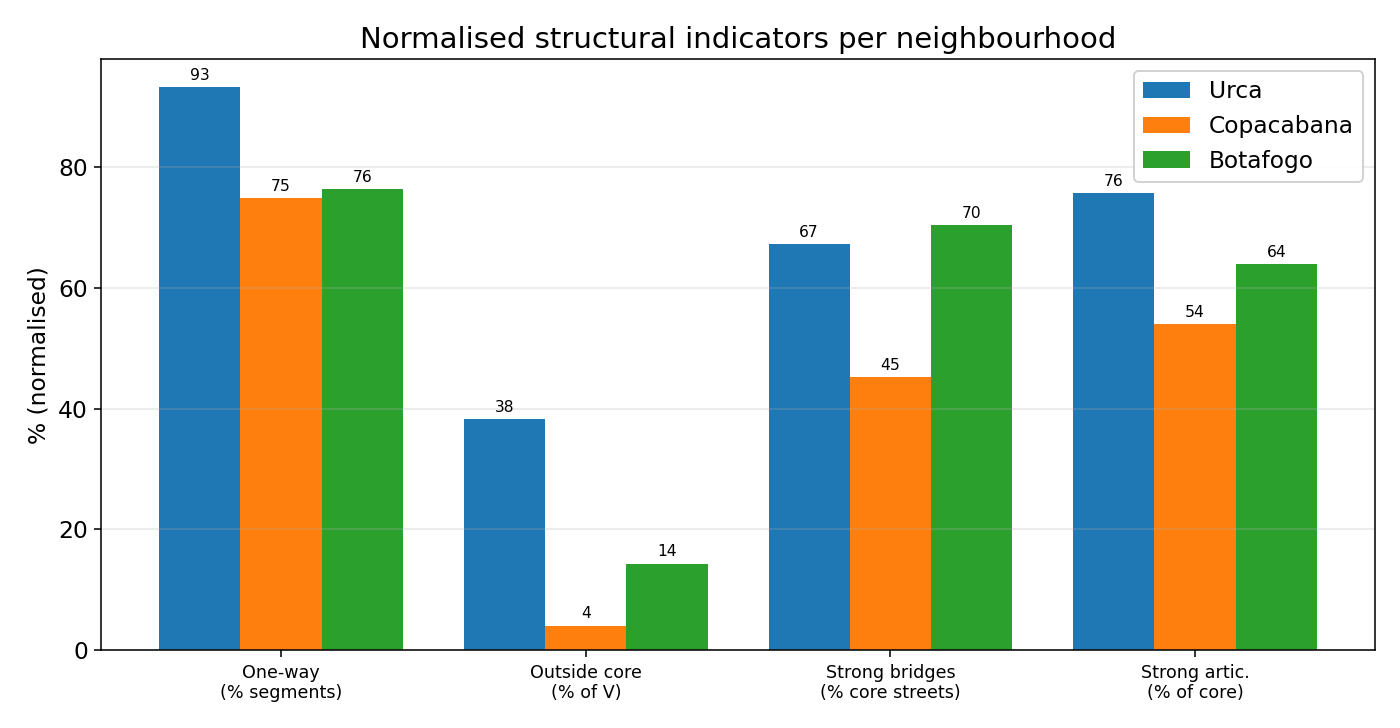
\includegraphics[width=\textwidth]{Figures/fig_comparison.png}
\caption{Indicadores estruturais normalizados por bairro, atualizados
para a rede corrigida de Copacabana. As proporções estruturais separam a
Urca das duas malhas abertas, mas deixam de equipará-las entre si; o
fluxo de acesso da Tabela~\ref{tab:acesso} é o que isola a porta única da
Urca.}
\label{fig:comparison}
\end{figure}
\FloatBarrier

% =====================================================================
\section{Conclusão}
\label{sec:conclusion}

Os indicadores estruturais tradicionais, pontes fortes e pontos de
articulação fortes, não separam os casos ao longo de um eixo de
gargalo: as duas malhas abertas permanecem distantes do regime da Urca,
mas, uma vez corrigida a rede de Copacabana para sua fronteira
administrativa oficial, as duas malhas abertas deixam de se assemelhar
tão de perto quanto sugeriria uma leitura não corrigida. O corte mínimo
entre dois nós é pouco informativo aqui, saturando em um porque malhas
de mão única densa contêm pontes não dirigidas por quase toda parte. O
sinal distintivo vem de um fluxo máximo entre o núcleo de cada bairro e
suas portas de acesso administrativas reais: a península se conecta ao
restante da cidade por uma única porta de acesso disjunta por ruas,
enquanto Copacabana oferece dezoito, e Botafogo, dezesseis. Um desvio
forçado ao redor de uma rua fechada também custa mais na Urca (13,6\% a
mais de tempo de percurso) do que em qualquer uma das malhas abertas
(5,1\% e 6,0\%). O gargalo de acesso é, assim, uma propriedade da
geografia da península, e não se generaliza para bairros grandes, nem
mesmo para um conhecido pela restrição de acesso por túneis. Essas
observações baseiam-se em $n=3$ casos contrastantes e são ilustrativas,
não estatisticamente gerais; estender a comparação a mais bairros,
correlacionar o fluxo de acesso com um índice geométrico de forma, e
conferir o máximo de intermediação contra um modelo nulo
(Seção~\ref{sec:discussion}) ficam para trabalhos futuros.

\subsubsection*{Reprodutibilidade.} Todo o código-fonte e os dados
estão abertamente disponíveis (repositório omitido para a revisão
duplo-cega).

% =====================================================================
\bibliographystyle{splncs04}
\bibliography{references}
% Bibliografia em references.bib. NOVAS entradas a acrescentar (ver
% aviso na resposta que acompanha este arquivo): hillier1984social,
% ipp_bairros.

\end{document}
